%!TEX program =pdflatex
\documentclass{beamer}
\usetheme{CambridgeUS}
%%define new comand
\def\argmin{\mathop{\rm arg~min}\limits}
\def\argmin{\mathop{\rm arg~min}\limits}
\newcommand{\bdelta}{\boldsymbol{\delta}}
\newcommand{\bbeta}{\boldsymbol{\beta}}
\newcommand{\bSigma}{\boldsymbol{\Sigma}}
\newcommand{\brho}{\displaystyle{\large{\boldsymbol{\rho}}}}
\newcommand{\bgamma}{\boldsymbol{\gamma}}
\newcommand{\bfeta}{\boldsymbol{\eta}}
\newcommand{\bPsi}{\boldsymbol{\Psi}}
\newcommand{\bmu}{\boldsymbol{\mu}}
\newcommand{\bvartheta}{\boldsymbol{\vartheta}}
\newcommand{\bzero}{\mathbf{0}}
\newcommand{\bone}{\mathbf{1}}
\newcommand{\bA}{\mathbf{A}}
\newcommand{\ba}{\mathbf{a}}
\newcommand{\bB}{\mathbf{B}}
\newcommand{\bb}{\mathbf{b}}
\newcommand{\bD}{\mathbf{D}}
\newcommand{\bU}{\mathbf{U}}
\newcommand{\bu}{\mathbf{u}}
\newcommand{\bV}{\mathbf{V}}
\newcommand{\bW}{\mathbf{W}}
\newcommand{\bw}{\mathbf{w}}
\newcommand{\bX}{\mathbf{X}}
\newcommand{\bx}{\mathbf{x}}
\newcommand{\bY}{\mathbf{Y}}
\newcommand{\by}{\mathbf{y}}
\newcommand{\bZ}{\mathbf{Z}}
\newcommand{\bz}{\mathbf{z}}
\newcommand{\suit}[1]{\left(#1\right)}
\newcommand{\abs}[1]{\left\vert#1\right\vert}
\newcommand{\set}[1]{\left\{#1\right\}}
\newcommand{\msuit}[1]{\left[ #1 \right]}
\author{Axel B\"ucher and Chen Zhou}
\title{A horse racing between the block maxima
method and the peak–over–threshold approach}
\begin{document}
\begin{frame}
\titlepage
\begin{center}
    Presented by Liujun Chen.
\end{center}
\end{frame}
\AtBeginSection[]
{
\begin{frame}
\frametitle{Table of Contents}
\tableofcontents[currentsection]
\end{frame}
}


\section{Introduction}
\begin{frame}
    \frametitle{Domain of Attraction Condition}
There exists a constant $\gamma\in \mathbb{R}$ and sequences $a_r>0$ and $b_r\in \mathbb{R}$ such that 
$$
\lim_{r\to \infty} F^r(a_rx +b_r)=\exp\suit{-(1+\gamma x)^{-1/\gamma}}\ \text{for all} \ 1+\gamma x>0. \quad (1.1)
$$

An equivalent representation of the domain of attraction condition is: there exists a positive function $\gamma=\sigma(t)$ such that 
$$
\lim_{t\to x^*}\frac{1-F(t+\sigma(t)x)}{1-F(t)}=(1+\gamma x)^{-1/\gamma} \ \text{for all} \ 1+\gamma x>0.\quad (1.2)
$$
\end{frame}


\begin{frame}
    \frametitle{BM}
Let $X_1,\dots,X_n$ be a sample of observations drawn
from F ( assume that the observations are independent {\color{blue} for the moment}). 

\begin{itemize}
    \item Divide the data into $k=[n/r]$ blocks of length $r$.
    \item By independence, each block maxima has cdf $F^r$.
    \item By (1.1), for large block sizes
    r, the sample of block maxima can then be regarded as an approximate i.i.d. sample from the three-parametric GEV:
    $$
        G_{\gamma,b,a}^{GEV}(x):=\exp\set{-(1+\gamma\frac{x-b}{a})^{-1/\gamma}}1\suit{1+\gamma\frac{x-b}{a}>0}.
    $$
    \item MLE $(\gamma>-1/2)$ or PWM $(\gamma<1/2)$.
\end{itemize}
    

\end{frame}



\begin{frame}
    \frametitle{POT}
Equation (1.2) gives rise to the competing peak-over-threshold approach (positive): for sufficiently large $t$ in (1.2), we obtain that, for any $x>0$,
$$
P(X>t+x|X>t) = \frac{P(X>t+x)}{P(x>t)}\approx (1+\gamma \frac{x}{\sigma})^{-1/\gamma}=:1-G_{\gamma,\sigma}^{GP}(x).
$$
\begin{itemize}
    \item In practice, $t$ is typically as the $n-k$th order statistics $X_{n-k,n}$ for some intermediate value $k$.
    \item Then, one may regard the sample $X_{n-k+1,n}-X_{n-k,k}, \dots, X_{n,n}-X_{n-k,n}$ as observations from the two parametric GPD.
    \item  MLE $(\gamma>-1/2)$, PWM $(\gamma<1/2)$, Hill $(\gamma>0)$, or Moment $(\gamma\in \mathbb{R})$
\end{itemize}

\end{frame}

\begin{frame}
    \frametitle{Outline of this paper}
    The goal of the present paper is an in-depth comparison of the two approaches.
\begin{itemize}
    \item Efficiency comparison in i.i.d. scenarios.
    \vspace{5ex}
    \item BM and POT applied to time series.
    \vspace{5ex}
    \item Extensions to multivariate observations and stochastic processes.
\end{itemize}
    

\end{frame}

\section{Efficiency Comparison for univariate i.i.d. observations}
\begin{frame}
    \frametitle{Efficiency Comparison}
\begin{itemize}
    \item The efficiency of BM and POT estimators can be compared in terms of their asymptotic bias and
    variance.
<<<<<<< HEAD
    \bigskip
=======
>>>>>>> 289f5da58f43f34b477429583765552fe477880e
    \item Particularly focus on the estimation of the extreme value index $\gamma$.
\end{itemize}
    

\end{frame}

\begin{frame}
    \frametitle{Efficiency Comparison}
    \begin{itemize}
    \item In both the BM and POT approach, a key tuning parameter is $k=k(n)$. (the number of blocks in the BM, the number
    of upper order statistics in the POT). {\color{red} Theoretically, $k=k(n)\to \infty,k/n\to 0$ as $n \to \infty$.}
    \item The asymptotic variance of the two estimators is of order $1/k$.
    \item The bias
    depends on how well the distribution of block maxima or threshold exceedances is approximated
    by the GEV or GP distribution, respectively.
\end{itemize}
    

\end{frame}

\begin{frame}
    \frametitle{Two Extreme Cases}
    Consider two extreme examples first (where the condition $k/n \to 0$ as $n \to \infty$ may in fact be discarded).
    \begin{itemize}
        \item For the Fr\'echet distribution, the block maximas of size $r=1$ ($k=n$) are already GEV-distributed. The convergence rate is $1/\sqrt{n}$ and the POT fails to achieve this rate.
        \item For the POT distribution, $k=n$ largest order
         statistics can be used for the estimation via POT. The rate of convergence for POT is $1/\sqrt{n}$.
    \end{itemize}
    

\end{frame}

\begin{frame}
    \frametitle{Second Order Condition}
    \begin{itemize}
        \item    Apart form these two (or similar) extreme cases, the optimal choice of $k$ depends on second order condition quantifying the speed of convergence in the DOA condition.
        \item They are formulated in terms of the two quantile functions 
        $$
            U(x)=\suit{\frac{1}{1-F}}^{\leftarrow}(x), \ V(x)=\suit{\frac{1}{-\log F}}^{\leftarrow}(x).
        $$
        for the POT- and the BM method, respectively.
    \end{itemize}
 
\end{frame}

\begin{frame}
    \frametitle{DOA condition for $U$ and $V$}
\begin{itemize}
    \item There exists a positive function $a_{POT}$ such that, for all $x>0$,
    $$
        \lim_{t\to\infty}\frac{U(tx)-U(t)}{a_{POT}(t)}=\int_{1}^x s^{\gamma-1}ds = \frac{x^{\gamma}-1}{\gamma}=:h_{\gamma}(x).
    $$
    \item There exists a positive function $a_{BM}$ such that, for all $x>0$,
    $$
    \lim_{t\to\infty}\frac{V(tx)-V(t)}{a_{BM}(t)}=\int_{1}^x s^{\gamma-1}ds = \frac{x^{\gamma}-1}{\gamma}=:h_{\gamma}(x).
    $$
\end{itemize}
The bias of certain BM- and POT estimators is determined by the speed of convergence in the
latter two limit relations, which can be captured by suitable second order conditions.
\end{frame}

\begin{frame}
    \frametitle{Second order conditions for $U$ and $V$}
    Define 
    $
        H_{\gamma,\rho}(x)=\int_{1}^x s^{\gamma-1} \int_{1}^s u^{\rho-1}duds.
    $
\begin{itemize}
    \item Suppose that there exists $\rho_{POT}\le 0$, a positive function $a_{POT}$ and a positive or negative function $A_{POT}$ with $\lim_{t\to\infty} A_{POT}=0$, such that for all $x>0$,
    $$
        \lim_{t\to \infty}\frac{1}{A_{POT}(t)}\suit{\frac{U(tx)-U(t)}{a_{POT}(t)}-h_{\gamma}(x)}=H_{\gamma,\rho_{POT}}(x)
    $$
    \item 
    Suppose that there exists $\rho_{BM}\le 0$, a positive function $a_{BM}$ and a positive or negative function $A_{BM}$ with $\lim_{t\to\infty} A_{BM}=0$, such that for all $x>0$,
    $$
        \lim_{t\to \infty}\frac{1}{A_{BM}(t)}\suit{\frac{V(tx)-V(t)}{a_{BM}(t)}-h_{\gamma}(x)}=H_{\gamma,\rho_{BM}}(x)
    $$
\end{itemize}
    

\end{frame}

\begin{frame}
    \frametitle{Remarks about the SOC}
\begin{itemize}
    \item THe functions $\abs{A_{BM}}$ and $\abs{A_{POT}}$ are then necessarily regularly varying with index $\rho_{BM}$ and $\rho_{POT}$ respectively.
    \item The limit distribution $H_{\gamma,\rho}$ appear specific, see e.g. de Haan and Ferreira (2006).
    \item If the     speed of convergence is faster than any power function, we set $\rho=-\infty$. For example, for GP family, the $\rho_{POT}=-\infty$; for GEV family, $\rho_{BM}=-\infty$.
\end{itemize}
    

\end{frame}

\begin{frame}
    \frametitle{$\rho_{BM}$ and $\rho_{POT}$}
    \begin{itemize}
        \item It is important to note that $\rho_{BM}$ and $\rho_{POT}$ can be vastly different. 
        \item A general result can be found in Drees, de Haan and Li (2003): If $2tA(t)\to c \in [-\infty,\infty]\backslash(1-\gamma)$, the two coefficients are equal within the range $[-1,0]$. Otherwise, if $\rho_{BM}<-1$, then $\rho_{POT}=-1$. If $\rho_{POT}<-1$, then $\rho_{BM}=-1$.
    \end{itemize}
    

    

\end{frame}

\begin{frame}
    \frametitle{$\rho_{BM}$ and $\rho_{POT}$}

    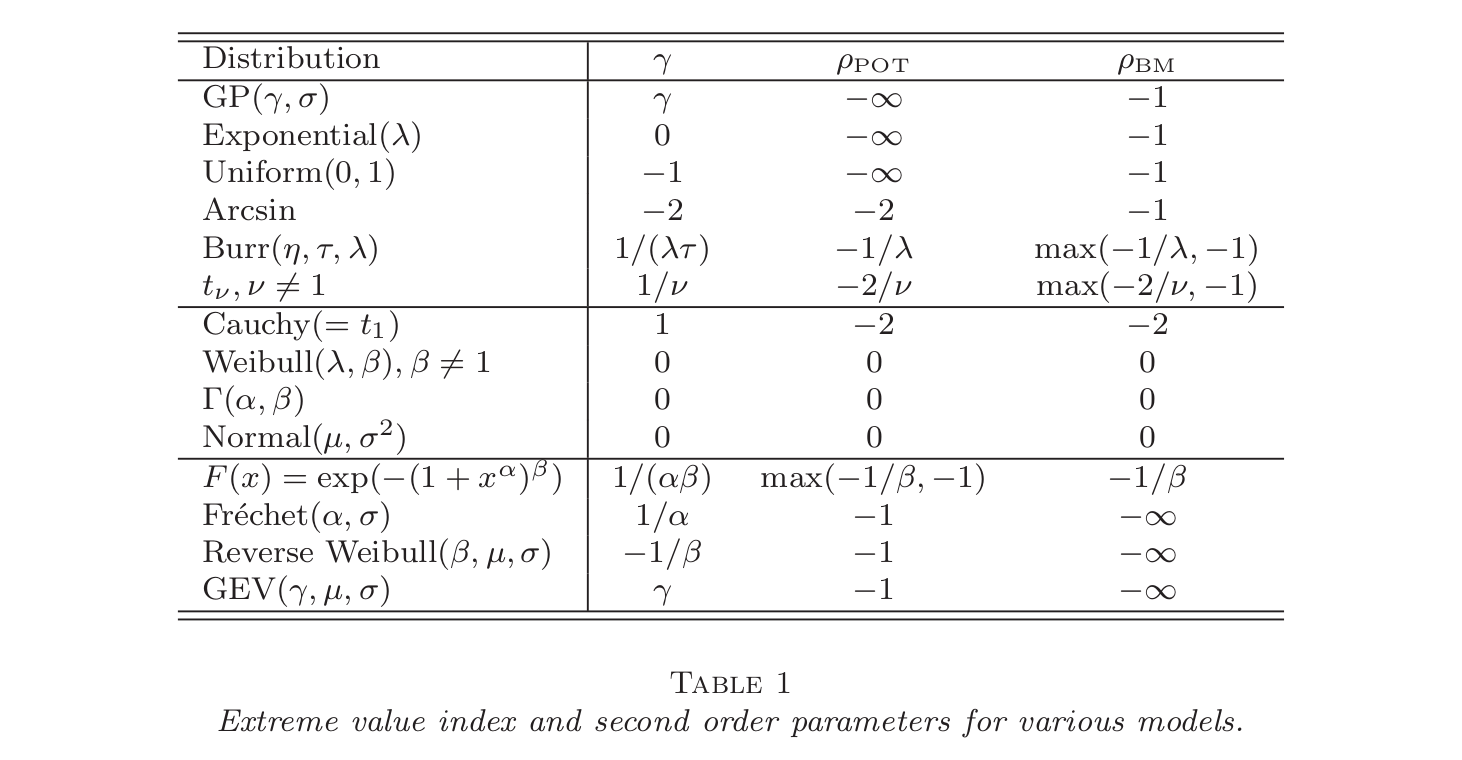
\includegraphics[width=1\textwidth]{fig1.png}

\end{frame}

\begin{frame}
    \frametitle{Asymptotic theory for the estimation of $\gamma$}
\begin{itemize}
    \item Solid theoretical studies regarding the POT method have a much longer history. For the sake of theoretical comparability with the BM
    method, we only deal with the MLE and the PWM.
    \item Perhaps surprisingly, asymptotic theory for the BM method has hitherto mostly ignored the fact that
    block maxima are only {\color{red} approximately} GEV distributed.
<<<<<<< HEAD
    \item Only recent theoretical studies in Ferreira and de Haan (2015) and Dombry and Ferreira (2019) for the PWM and MLE, respectively,
=======
    \item Only recent theoretical studies in Ferreira and de Haan (2015) and Dombry and Ferreira (2017) for the PWM and MLE, respectively,
>>>>>>> 289f5da58f43f34b477429583765552fe477880e
    take the approximation into account.
\end{itemize}
\end{frame}

\begin{frame}
    \frametitle{Asymptotic theory for the estimation of $\gamma$}
    Under the respective second order conditions for $U$ and $V$, the asymptotic result can be summarized as 
    $$
\hat{\gamma}\stackrel{d}{\approx} N\suit{\gamma+A_m(n/k)b,\frac{1}{k}\sigma^2}, \ m \in \set{BM,POT}.
    $$
    
    Here, the asymptotic bias $b$ and the asymptotic variance depend on the specific estimator, $\rho_m$ and $\gamma$. In particular,
    the rate of convergence of the bias $A_m(n/k)$ crucially depends on the second order index $\rho_m$.

\end{frame}

\begin{frame}
    \frametitle{Rate of convergence}
We consider the rate of convergence of the root mean squared error.

\begin{itemize}
<<<<<<< HEAD
    \item Assume that $A_m(t) \asymp t^{\rho_m}$ with $\rho_m\in (-\infty,0)$.
    \item The best attainable
    rate of convergence is achieved when squared bias and variance are of the same order, that is, when 
    $$
        A_m^2\suit{\frac{n}{k}} \asymp \suit{\frac{n}{k}}^{2\rho_m} \asymp \frac{1}{k}.
    $$
    \item Solving for $k$ yields $k \asymp n^{-2\rho_m/(1-2\rho_m)}$, which implies
=======
    \item Assume that $A_m(t)=t^{\rho_m}$ with $\rho_m\in (-\infty,0)$.
    \item The best attainable
    rate of convergence is achieved when squared bias and variance are of the same order, that is, when 
    $$
        A_m^2\suit{\frac{n}{k}} = \suit{\frac{n}{k}}^{2\rho_m}=\frac{1}{k}.
    $$
    \item Solving for $k$ yields $k=n^{-2\rho_m/(1-2\rho_m)}$, which implies
>>>>>>> 289f5da58f43f34b477429583765552fe477880e
    $$
\text{Rate of convergence of} \ \hat{\gamma} = n^{-2\rho_m/(1-2\rho_m)},
    $$
    irrespective of $m \in \set{POT,BM}$.
\end{itemize}
    

\end{frame}

\begin{frame}
    \frametitle{Convergence Rate}
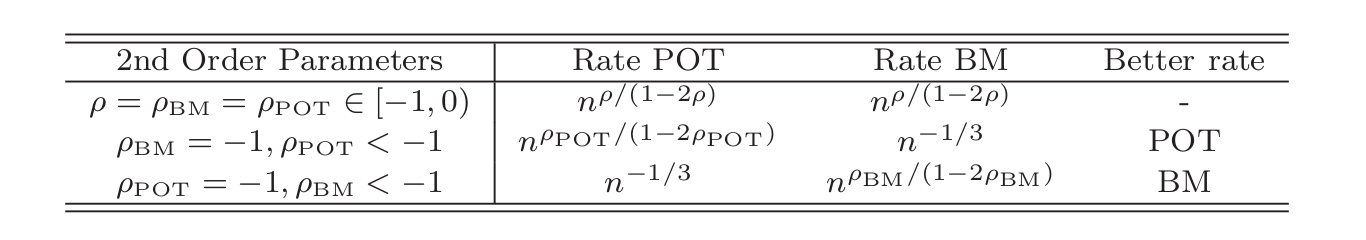
\includegraphics[width=1\textwidth]{fig2.png}
    
\begin{itemize}
    \item For $\rho_m=-\infty$, the convergence rate is 'faster than $n^{-1/2+\varepsilon}$ for any $\varepsilon>0$'. And depending on the underlying distribution, in fact could even achieve $n^{-1/2}$.
\end{itemize}
\end{frame}


\begin{frame}
    \frametitle{Asymtotic mean squared error}
\begin{itemize}
    \item If $\rho_{POT}\ne \rho_{BM}$, the approach corresponding to a lower $\rho$ generally yields estimators for $\gamma$ with a faster attainable rate of convergence than the other approach.
    \item In this subsection, we consider the case $\rho_{BM}=\rho_{POT}$.
    \item Hence, the efficiency comparison should be made at the level of asymptotic mean squared error
    (AMSE) or, more precisely, its two subcomponents: asymptotic bias and asymptotic variance.
\end{itemize}
    

\end{frame}

\begin{frame}
    \frametitle{Asymtotic mean squared error}

    \begin{itemize}
        \item A detailed analysis of the PWM and the ML estimators under the BM and POT approach has
<<<<<<< HEAD
        been carried out in Ferreira and de Haan (2015) and Dombry and Ferreira (2019), for the case $\rho_{BM}=\rho_{POT}=[-1,0]$ and $\gamma\in (-0.5,0.5)$.
=======
        been carried out in Ferreira and de Haan (2015) and Dombry and Ferreira (2017), for the case $\rho_{BM}=\rho_{POT}=[-1,0]$ and $\gamma\in (-0.5,0.5)$.
>>>>>>> 289f5da58f43f34b477429583765552fe477880e
        \item When using the same value for $k$, the BM version of either ML or PWM     leads to a lower asymptotic         variance compared to the corresponding POT version, for all $\gamma\in (-0.5,0.5)$.
        \item Asymptotic bias is smaller for the POT versions of the two estimators, for all $(\gamma,\rho)\in (-0.5,0.5)\times [-1,0]$.
        \item When comparing the optimal AMSE, for the ML, POT is better. For the PWM, BM is preferable for most combinations of $(\gamma,\rho)$.
    \end{itemize}

\end{frame}


\begin{frame}
    \frametitle{Threshold and block length choice}
\begin{itemize}
    \item Both the POT and the BM approach require a practical selection for the intermediate sequence $k=k_n$ in a sample of size $n$.
    \item In the POT approach, the choice of $k$ can be interpreted as
    the choice of the threshold above which the POT approximation s regarded as sufficiently
    accurate.
    \item Similarly, in the BM approach, $k$ is related to $r=n/k$, which is the size of the block
    of which the GEV approximation to the block maximum is regarded as sufficiently accurate.
\end{itemize}
    

\end{frame}


\begin{frame}
    \frametitle{Threshold and block length choice}

    \begin{itemize}
        \item The theoretical conditions that $k\to \infty$ and $k/n\to 0$, as $n \to 0$, are useless in guiding the practical choice. 
        \item Practically, often a plot between the estimates based on various k against the values
        of k is made for resolving this problem, the so-called “Hill plot”.
        \item The Hill plot can be also be applied to other POT or even BM estimators than
        just the Hill estimator.
        \item The ultimate choice is then made by taking a $k$ from the first stable
        region in the “Hill plot”. Nevertheless, the estimators are often rather sensitive to the choice of $k$.
    \end{itemize}

\end{frame}

\begin{frame}
<<<<<<< HEAD
    \frametitle{The choice of $k$}
=======
    \frametitle{The choice of $k$ for the POT}
>>>>>>> 289f5da58f43f34b477429583765552fe477880e
    For the POT approach, there exist a few attempts on resolving the choice of k issue in a formal manner.
\begin{itemize}
    \item One solution is to find the optimal k that minimizes the asymptotic MSE; see, e.g., Danielsson et al. (2001), Drees and Kaufmann (1998) and Guillou and Hall (2001).
    \item one may also rely on bias corrections, which typically allows
    for a much larger choice of $k$, see e.g., Gomes, De Haan and Rodrigues (2008).
\end{itemize}
<<<<<<< HEAD
\medskip

For the BM approach: unknow till now.
=======
    
>>>>>>> 289f5da58f43f34b477429583765552fe477880e

\end{frame}


<<<<<<< HEAD

=======
\begin{frame}
    \frametitle{The choice of $k$ for the BM}
    \begin{center}
        Unknown Till now.
    \end{center}

    

\end{frame}
>>>>>>> 289f5da58f43f34b477429583765552fe477880e

\section{BM and POT for Univariate Stationary Time Series}
\begin{frame}
    \frametitle{Extremes for Stationary Time Series}
\begin{itemize}
    \item Assume that $\suit{X_t}_{t\in \mathbb{Z}}$ is a strictly stationary univariate time series, and the
    stationary cdf F satisfies the domain-of-attraction condition.
<<<<<<< HEAD
    \bigskip
=======
>>>>>>> 289f5da58f43f34b477429583765552fe477880e
    \item It is important to note that
    the parameters $\gamma,a_r,b_r$ only depend on the stationary cdf $F$.
\end{itemize}
    

\end{frame}


\begin{frame}
    \frametitle{The POT approach for time series}

\begin{itemize}
    \item    Recall that the POT approach is based on the sample of large order statistics denoted by $\mathcal{X}_{POT}=\set{X_{n-k,n},\dots, X_{n,n}}$.
    \item Bearing in mind that, under mild extra conditions on the serial
    dependence (ergodicity, mixing conditions,...), empirical moments are consistent for their theoretical counterparts.
    \item Thus, we can still use PWM and MLE.
    \item The asymptotic variance of such estimators will however
    be different from the i.i.d. case in general.
\end{itemize}
\end{frame}

\begin{frame}
    \frametitle{The POT approach for time series}
\begin{itemize}
    \item Respective theory can be found in Hsing (1991); Resnick and Stărică (1998) for the Hill estimator and in Drees (2000) for a large class of estimators, including PWM and ML.
    \item Most of the
    estimators have the same bias as in the i.i.d. case, whereas their asymptotic variances depend
    on the serial dependence structure and are usually higher than those obtained in the i.i.d. case.
    \item Since the asymptotic bias shares the same explicit form, bias correction can also be performed
    in the same way as in the i.i.d. case; see, e.g., de Haan, Mercadier and Zhou (2016).
\end{itemize}
    

\end{frame}

\begin{frame}
    \frametitle{The BM approach for time series}
\begin{itemize}
    \item Recall that the BM approach is based on the sample of block maxima $\mathcal{X}_{BM}=\set{M_{1,r},\dots,M_{k,r}}$, where $M_{j,r}$ denotes the maximum within the jth disjoint block of observations of size $r$.
    \item The main
    motivation lead us to consider this sample as approximately GEV-distributed   was the relation
    $$
P\suit{M_{1,r}\le a_r x+b_r}=F^r(a_r x+b_r)\approx G^{GEV}_{\gamma,0,1}(x),
    $$
    for large $r$. 
    \item The first equality is not true for time series, whence more sophisticated arguments
    must be found for the BM method to work for time series.
\end{itemize}
    

\end{frame}

\begin{frame}
    \frametitle{The BM approach for time series}
\begin{itemize}
    \item   If $F$ satisfies the DOA condition, and some mixing condition on the serial dependence are met, then there exists a constant $\theta \in[0,1]$ such that
    $$
    P\suit{M_{1,r}\le a_r x+b_r}\to\suit{G^{GEV}_{\gamma,0,1}(x)}^{\theta}.
    $$
     \item The constant $\theta$ is called the extremal index and can be interpreted as capturing the tendency of the time series that extremal observations occur in clusters.
\end{itemize}
    

\end{frame}


\begin{frame}
    \frametitle{Extremal Index}
If $\theta<0$, then letting
$$
\tilde{a}_r =a_r\theta^{\gamma}, \tilde{b}_r=b_r-a_r\frac{1-\theta^{\gamma}}{\gamma},
$$
we immediately obtain that
$$
P\suit{M_{1,r}\le \tilde{a}_r x+\tilde{b}_r}\to G^{GEV}_{\gamma,0,1}(x).
$$
\end{frame}

\begin{frame}
    \frametitle{Estimation of the extremal index}
\begin{itemize}
    \item 1) BM-like estimators based on “blocking”
    techniques (Northrop, 2015; Berghaus and Bücher, 2017)
    \item 2) POT-like estimators that rely on
    threshold exceedances (Ferro and Segers, 2003; Süveges, 2007)
    \item  3) estimators that use both principles simultaneously (Hsing, 1993; Robert, 2009; Robert, Segers and Ferro, 2009)
    \item 4) estimators which, next to choosing a threshold sequence, require the choice of a run-length parameter
    (Smith and Weissman, 1994; Weissman and Novak, 1998).
\end{itemize}
\end{frame}


\begin{frame}
    \frametitle{BM for time series}
\begin{itemize}
    \item Since the distance between the time points at which the maxima within two successive blocks
    are attained is likely to be quite large, the sample $\mathcal{X}_{BM}$ can be regarded as approximately independent.
    \item As a matter of fact, the literature on statistical theory for the BM method is mostly
    based on the assumption that $\mathcal{X}_{BM}$ is a genuine i.i.d. sample from the GEV-family.
    \item Two approximation errors are thereby completely ignored: the cdf is only approximately
    GEV, and the sample is only approximately independent.
\end{itemize}
    

\end{frame}

\begin{frame}
    \frametitle{BM for time series}

\begin{itemize}
    \item Solid theoretical results taking these
    errors into account are rare: Bücher and Segers (2018b) treat the ML-estimator in the heavy-
    tailed case ($\gamma>0$).
    \item The main conclusions are: the sample can safely be regarded as independent,
    but a bias term may appear which, similar as in Section 2, depends on the speed of convergence.(SOC)
    \item Bücher and Segers (2018a) improve upon that estimator by using sliding blocks instead
    of disjoint blocks. 
    \item The asymptotic variance of the estimator decreases, while the bias stays the
    same. Moreover, the resulting ‘Hill-Plots’ are much smoother, guiding a simpler choice for the
    block length parameter.
\end{itemize}

\end{frame}


\begin{frame}
    \frametitle{Comparisons}

    \begin{itemize}
        \item Due to the lack of a general theoretical result on the BM method, a theoretical comparison on 
        which method is more efficient seems out of reach for the moment.
        \item However, some insight into the merits and pitfalls of two approaches can be
        gained by considering the problem of estimating high quantiles and return levels.
    \end{itemize}

\end{frame}


\begin{frame}
    \frametitle{Estimating high quantiles}
For the BM,
$$
F^{\leftarrow}(1-p)\approx b_r+a_r\frac{\set{-r\log(1-p)}^{-\gamma}-1}{\gamma}\approx b_r+a_r\frac{(rp)^{-\gamma}-1}{\gamma}.
$$
For the POT,
$$
F^{\leftarrow}(1-p)\approx t+\sigma(t)\frac{(\frac{p}{1-F(t)})^{-\gamma}-1}{\gamma}.
$$
As a consequence, based on the plug-in principle, the POT method immediately
yields estimators for high quantiles On the other hand, the BM method cannot be used straight forwardly. It requires the estimation for $\theta$.
\end{frame}

\begin{frame}
    \frametitle{Estimating return levels}
Let $F_r(x)=P(M_{1,r}\le x)$. For $T\ge 1$, the T -return level of the sequence of block maxima is defined as the $1-1/T$ quantile of $F_r$, that is
$$
RL(T,r)=F_r^{\leftarrow}(1-1/T).
$$
    
We have that 
$$
RL(T,r) \approx \tilde{b_r}+\tilde{a_r}\frac{(r/T)^{-\gamma}-1}{\gamma}.
$$
Following the
discussion in the previous section, it is now the BM method which yields simpler estimators that
do not require additional estimation of the extremal index.
\end{frame}

\section{BM and POT for Multivariate Observations}

\begin{frame}
    \frametitle{Multivariate Extremes}
    suppose that there exists a non-degenerate cdf G and sequences $(a_{r,j})_{r\in \mathbb{N}}$, $(a_{r,j})_{r\in \mathbb{N}}$, $j=1,\dots,d$ with $a_{r,j}>0$ such that
    $$
    \begin{aligned}
&\lim_{r\to \infty}P\suit{\frac{\max_{i=1}^r X_{i,1}-b_{r,1}}{a_{r,1}}\le x_1,\dots,\frac{\max_{i=1}^r X_{i,d}-b_{r,d}}{a_{r,d}}\le x_d}\\
&=G(x_1,\dots,x_d).
    \end{aligned}
    $$
    The dependence between the coordinates of G can be described in various equivalent ways:
\begin{itemize}
    \item by the stable tail dependence function $L$ (Huang, 1992), 
    \item by
    the exponent measure $\mu$ (Balkema and Resnick, 1977), 
    \item by the Pickands dependence function $A$
    (Pickands, 1981), 
    \item by the tail copula $\Lambda$ (Schmidt and Stadtmüller, 2006),
    \item  by the spectral mea-
    sure $\Phi$ (de Haan and Resnick, 1977),
    \item by the madogram $\nu$ (Naveau et al., 2009),
\end{itemize}
    

\end{frame}



\begin{frame}
    \frametitle{Multivariate Extremes}
\begin{itemize}
    \item  Often, estimation of the marginal parameters and of the dependence structure is
    treated successively.
    \item  Standard errors for estimators of the dependence
    structure may then be influenced by standard errors for the marginal estimation, ( a point which
    is often ignored in the literature on statistics for multivariate extremes.)
\end{itemize}


\end{frame}

\begin{frame}
    \frametitle{The POT method in the multivariate case}
Based on observations 
$$
\mathcal{X}_{POT}=\set{\bX_i| \text{rank}(X_{i,j} \ \text{among}\  X_{1,j,\dots,X_{n,j}})\ge n-k  \ \text{for some}\ j=1,\dots,d}
$$
e.g. The estimation for the $L$ function.

Bias correction for $\hat{L}$ function have been proposed in in Fougères et al. (2015).

\end{frame}

\begin{frame}
    \frametitle{The BM method in the multivariate case}
    \begin{itemize}
        \item    Let $r$ denote a block size, and $k = [n/r]$
        the number of blocks.
        \item For $l=1,\dots,k$, let $\mathbf{M}_{l,r}=(M_{l,1,r},\dots,M_{l,d,r})^{'}$ denote the vector of componentwise block maxima.
        \item  Any estimator defined in terms of the sample $\mathcal{X}_{BM}=\set{\mathbf{M}_{1,r},\dots,\mathbf{M}_{k,r}}$ is called an estimator based on the BM approach.
        \item Just as for the univariate BM method, asymptotic theory is usually formulated under the assumption that $M_{1,r},\dots,M_{k,r}$ are iid sample from the limiting distribution $G$.
        \item Moreover, estimation of the marginal parameters is often
        disentangled from estimation of the dependence structure, with theory for the latter either developed under the assumption that marginals are completely known.
    \end{itemize}
 
    
    
    
    

\end{frame}

\begin{frame}
    \frametitle{Conclusion}
    \begin{center}
        There is no winner.
    \end{center}

    

\end{frame}
\end{document}